\documentclass{article}
\usepackage{fancyhdr,graphicx}
\setlength{\headheight}{15.2pt}
\pagestyle{fancy}
\begin{document}
\rhead{\fancyplain{}Page {\thepage}}
\lhead{\fancyplain{}Section {\thesection}}
\title{Bioinformatics Analysis of Effect of Hydrogen Peroxide on \emph{Beta vulgaris} Seeds}
\author{Vinay Hiremath \\ Dr. Mitch McGrath}
\date{16 July 2012}
\maketitle

\section{Introduction}
	It has recently been found through preliminary experiments that various types of seeds of the species \emph{Beta vulgaris} germinate significantly more successfully when placed in a solution of 0.3\% hydrogen peroxide (H$_{2}$O$_{2}$) as opposed to a solution of pure water (H$_{2}$O). The sugar beet crop contributes to approximately 20\% of global sugar production, and as a result, it is an important crop that people everywhere depend on for successful harvests. In the H$_{2}$O$_{2}$ solution, there is a noticeable difference in both germination time (shorter) and the percentage of seeds (higher) that are germinated after four days. It is likely that this change in success rates is a direct effect of a change in the genes being expressed by these seeds, and this phenomenon likely reflects the relative emergence potential of the varieties of sugar beet. After obtaining DNA sequences of the seeds in both the control and experimental group, I will attempt to use various bioinformatic tools in conjunction to arrive at a result that clearly expresses the specific DNA sequences that are expressed only in the experimental (H$_{2}$O$_{2}$) group. These tools employ RNA-Seq analysis methods (high-throughput mRNA sequencing).
\section{Hypothesis}
	As a result of the extensive procedure necessary to properly sequence the DNA of the trial groups, the limited data to be analyzed may be slightly lacking in scope. However, by comparing the genes only expressed in the experimental with annotated genomes for both \emph{Beta vulgaris} and other similar organisms, it is hopeful to maintain that the isolated expressed DNA sequences have similar listed roles in these genomes. Through this assimilation of previously gathered data, the expression of certain genes to affect the success rate of germination of the various seeds should become clear after extensive gene analysis.
\section{Methods}
	I will be using a large suite of bioinformatics tools, all of which are open-sourced under the GNU Public License as freely redistributable. Annotated genome data will be collected from sources using the Basic Local Alignment Search Tool (BLAST) through databases such as the Arabidopsis Information Resource (TAIR) and the Kyoto Encyclopedia of Genes and Genomes (KEGG), among others. The BLAST system finds ``regions of local similarity between protein or nucleotide sequences," as it calculates the statistical similarities of the matches (Bergman et al.). Queries to the BLAST are character strings of nucleotide or amino acid codes, often represented with a descriptive line in the FASTA format, which is further explained below. The alignment score is found by ``assigning a value to each aligned pair of letters"  and then adding these values along the alignment (Bergman et al.).\\\\
	In order to first build an index for the sequence files so that they can be more easily indexed, I first needed to generate detailed quality reports, so I used the fastqc toolset. This suite handles the FASTQ format, which is a text-based sequence for storing sequence data. It is the successor to the FASTA format, and its main difference is that it incorporates quality scores in the Phred format (Trapnell et al.). Next, I used a tool called bowtie2 as it enables strong compatibility with the assembly program I used, known as tophat. Using this suite of programs, I was able to assemble the data I had gathered onto the RefBeet 0.9 genome, made by the Max Planck Institute for Molecular Genetics. These alignments are reported in BAM files, a binary compressed version of the SAM format, together making up the predominant output formats of next-generation sequence alignment tools (Trapnell et al.). After this, I was able to analyze the remaining assembled data sets using the cufflinks suite. Cufflinks generated transcript indexes of each data set for both H$_{2}$O and H$_{2}$O$_{2}$ of each seed variety. Next, cuffdiff was able to find the sections of each contig that was different between the experimental and control data sets while avoiding those similar between the seed variety data sets, which helped to eliminate extraneous results. To convert these contigs to actual sequences as represented in the RefBeet genome, I made a custom script that extracts the base sequences from the reference genome by applying the contig number and position given by cuffdiff. After these sequences were found and input into a text file, I submitted them to a large variety of BLAST databases as previously listed. The annotated databases output predicted roles of each difference between the control and experimental data sets. Through the Cufflinks output, I was also able to generate detailed expression plots such as volcano, scatter, and box plots using tool called CummeRbund. This tool parses the Cufflinks output into R objects, which are more suitable for data analysis because of the wide variety of R packages available for this purpose.

\section{Application}
	When properly applied, the gene sequences that are found to be expressed by \emph{Beta vulgaris} seeds as a result of H$_{2}$O$_{2}$ can then be used to simulate similar growth in seeds that have not been soaked in this solution. The importance of this result lies in the fact that an H$_{2}$O$_{2}$ solution, although helpful for seed germination, harms further plant development. As a result, it is important to isolate the successful factors of the seeds in this solution without exposing the plant to the solution itself. This application has the potential to revolutionize sugar beet growth in a variety of environments that require more successful and quicker seed germination.

\section{Initial Results}

\subsection{FASTQC Format Example}
	This example is from the MSR3 data set soaked in water. As described, the FASTQ format bundles quality scores, which are displayed on the \textbf{fourth line}. The \textbf{first line} is a systematic identifier created by the Illumina sequencing system, while the \textbf{second line} is the raw sequenced bases and the \textbf{third line} is an optional description line. Excerpts of two sample sequences are shown here. \\
\begin{verbatim}
@HWI-ST957:100:D0V52ACXX:5:1101:1226:2111 1:N:0:CAGATC
GTGGGCATGAAGTGTGGGGATAGCATGGACTCGCCAGTTGTATCGGCGGTCGTGGGGGAGGGGGGC...
+
;?@DFDDAHFDDAEAEHIICCCEHHDIJEHJJIJJHGFHHIIJGGIIIF#################...

@HWI-ST957:100:D0V52ACXX:5:1101:1219:2188 1:N:0:CAGATC
GTGAGCATACCTGTCGGGACCCGAAAGATGGTGAACTATGCCTGAGCGGGGCGAAGCCAGAGGAAA...
+
@BBADBDEFHHHHGEEHIGGIJHCDBG?FGGDGGGGGFGHBFGHCGGHGID?@559BB<<2<@28A...
\end{verbatim}


\subsection{Sequence Output Information}
	These data graphs represent the Phred quality scores output from the Illumina Genome sequencing system. They are created using the FASTQC toolkit, which handles the FASTQ format. The graphs show the quality along each 100bp read of the full sequence, as the sequencing machines that were used handle 100bp reads. This representation is ideal to identify a read error in the machine, because a dramatic drop in quality in one particular position of the read indicates the same problem in each run of the machine.
\newpage
MSR3 set in water: \\
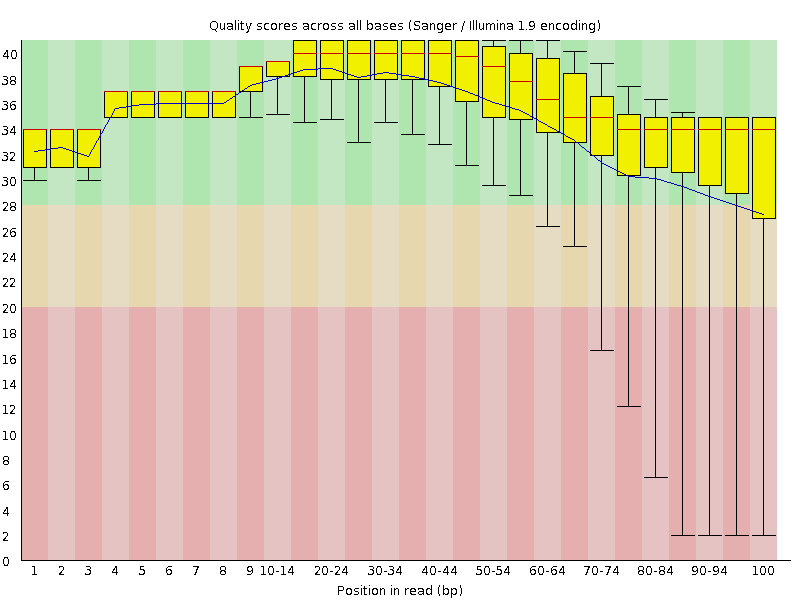
\includegraphics[scale=0.3]{msr3_h20_r1_basequal.png} \\
	\begin{tabular}{| l | r |}
	\hline
	Total sequences & 24155194 \\ \hline
	Sequence length & 100bp \\ \hline
	GC content & 48\% \\ \hline
	\end{tabular} \linebreak
\\
MSR3 set in hydrogen peroxide: \\
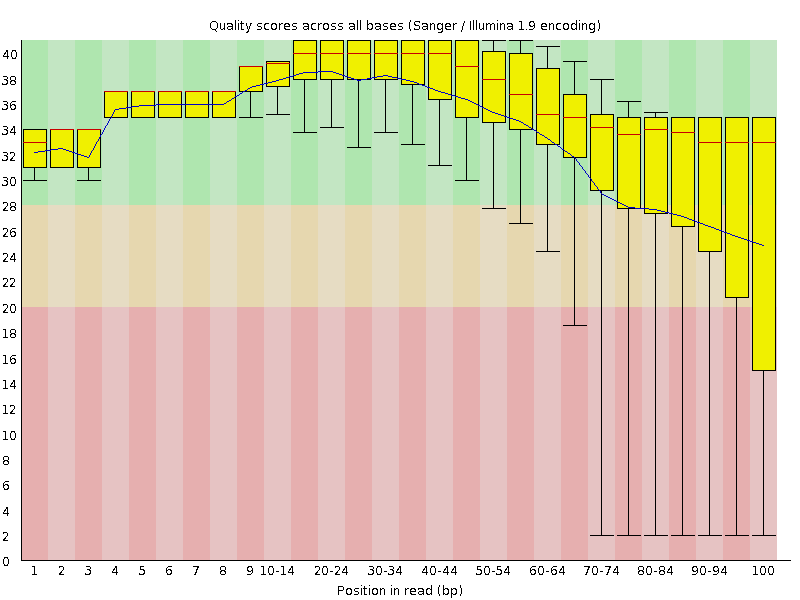
\includegraphics[scale=0.3]{msr3_h202_r1_basequal.png} \\
	\begin{tabular}{| l | r |}
	\hline
	Total sequences & 25694416 \\ \hline
	Sequence length & 100bp \\ \hline
	GC content & 49\% \\ \hline
	\end{tabular} \linebreak
\newpage
USH20 set in water: \\
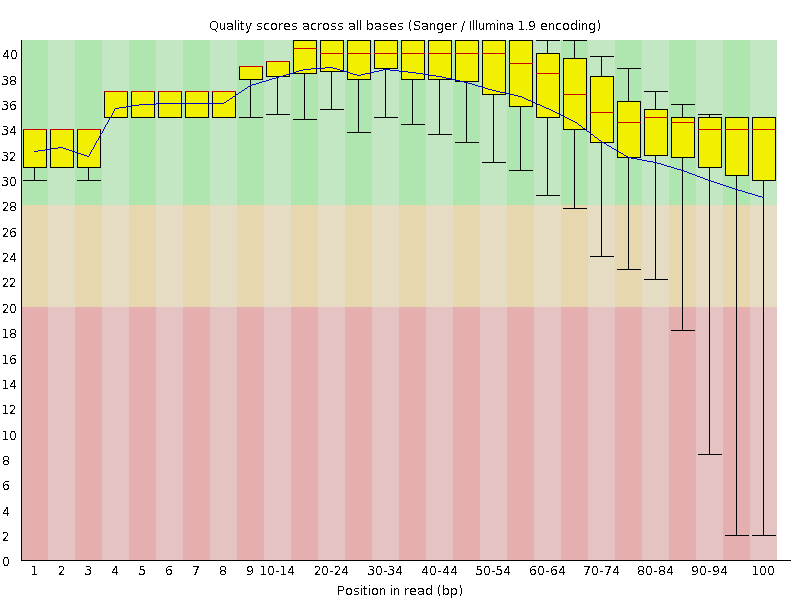
\includegraphics[scale=0.3]{ush20_h20_r1_basequal.png} \\
	\begin{tabular}{| l | r |}
	\hline
	Total sequences & 28485306 \\ \hline
	Sequence length & 100bp \\ \hline
	GC content & 44\% \\ \hline
	\end{tabular} \linebreak
\\
USH20 set in hydrogen peroxide: \\
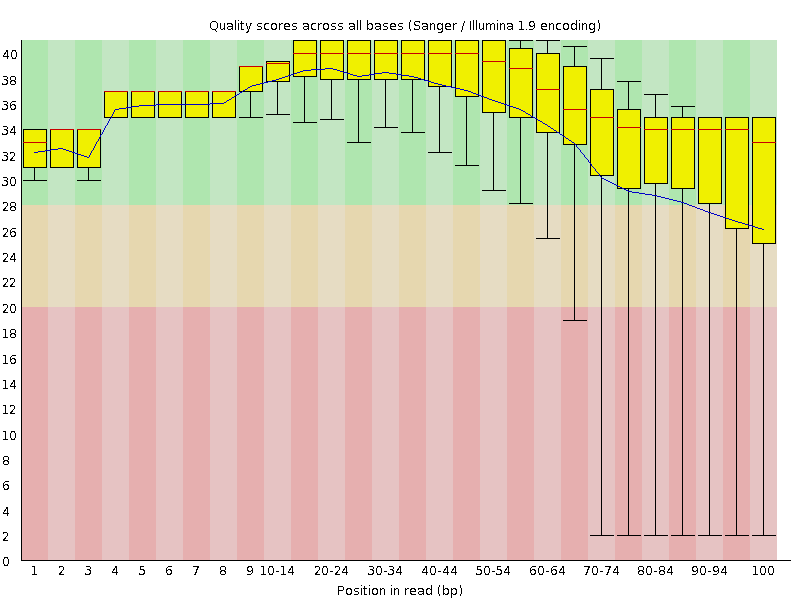
\includegraphics[scale=0.3]{ush20_h202_r1_basequal.png} \\
	\begin{tabular}{| l | r |}
	\hline
	Total sequences & 23853050 \\ \hline
	Sequence length & 100bp \\ \hline
	GC content & 45\% \\ \hline
	\end{tabular} \linebreak
\newpage
% \subsection{Bowtie2 Index Information for MSR3:}

\subsection{Genome Processing File Sizes:}

	\begin{tabular}{| l | c | c | c | r |}
	\hline
	Genome Name & File Size & Bowtie2 Index & Tophat Index & Cufflinks Index\\ \hline
	RefBeet 0.9 & 601906023B, 575MB & 719MB & TBD & TBD \\ \hline
	SAMS & 6261667B, 6.0MB & 17.3MB & TBD & TBD \\ \hline
	\end{tabular}
\newline

%\section{Data Processing}



%\subsection{Cufflinks Index Information:}

%\subsection{Cuffdiff Output Information:}



%\subsection{Example of BLAST Database:}

\newpage
\section{Works Cited}

Trapnell, Cole, Adam Roberts, Loyal Goff, Geo Pertea, Daehwan Kim, David R. Kelley, Harold Pimentel, Steven L. Salzberg, John L. Rinn, and Lior Pachter. ``Differential Gene and Transcript Expression Analysis of RNA-seq Experiments with TopHat and Cufflinks." Nature Protocols 7 (2012): 562-78. Nature Protocols. Nature, 01 Mar. 2012. Web. 15 July 2012. \\ \\
Bergman, Nicholas H., David Wheeler, and Medha Bhagwat. Comparative Genomics. Vol. 1-2. Totowa, NJ: Humana, 2007. Print.

\end{document}
